

\section{Results}\label{sec:result}
All the following simulations were implemented in Simulink, using fourth order Runge-Kutta algorithm with fixed step size of $0.001$.
\subsection{Model Validation}
Before proceeding with further analysis, the model in analysis must be tested and compared with known results.

The comparison will be done with 2 different authors. First, R\"ossler original paper \cite[Fig. 2]{rossler1976equation} will be used as reference. R\"ossler firstly proposed the model using $a=b=0.2$ and $c=5.7$ with initial conditions $(x_{10},x_{20},y_{0})=(0,-6.78,0.02)$.
Thus, the parameters for our circuit simulation will be $u(t)=0V$, $V_{cc0}=15V$, $RC=1s$, $R_a=500k\Omega$, $R_b=7500k\Omega$, $R_c=17.5934k\Omega$, with $t_0=0s$ and $t_{\text{end}}=339.249s$. The results of the simulation are shown in Fig. \ref{fig:validRoss}.

\begin{figure}[H]
    \centering
    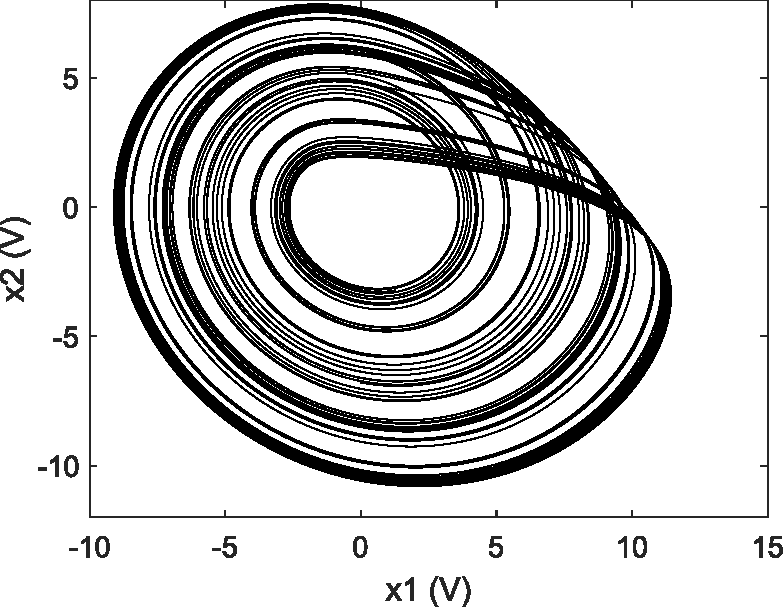
\includegraphics[scale=0.4]{figs/x1vsx2ValidRoss.pdf}
    \caption{Phase portrait results of $x_2x_1$ plane using R\"ossler \cite{rossler1976equation} parameters.}
    \label{fig:validRoss}
\end{figure}

This figure shows the trajectory followed by the system between $t=0$ and $t=339.249$, note that it follows an enclosed trajectory but not necessarily periodic; note as well the Möbius strip-like behavior, as Rössler states in his main paper \cite{rossler1976equation}.

On the other hand, Sprott and Li presented useful simulations for R\"ossler system, providing results for both phase portraits and time responses of the state variables \cite[Figs. 2 and 3]{sprott2017asymmetric}. The simulations were done with $a=0.29$, $b=0.14$ and $c = 4.52$, with two initial conditions: $IC1 = (-1.25, -0.72, -0.10)$ and $IC2 = (0.72,1.28,0.21)$. Thus, our circuit parameters are $u(t)=0V$, $V_{cc0}=15V$, $RC=1s$, $R_a=344.8276k\Omega$, $R_b=10714k\Omega$, $R_c=22.1239k\Omega$, with $t_0=0s$ and $t_{\text{end}}=100s$.

The results for the phase portraits are shown in Fig. \ref{fig:validPhase} and for the time responses in Fig. \ref{fig:validTime}.
\begin{figure*}
        \centering
        \begin{subfigure}[b]{0.3\textwidth}
            \centering
            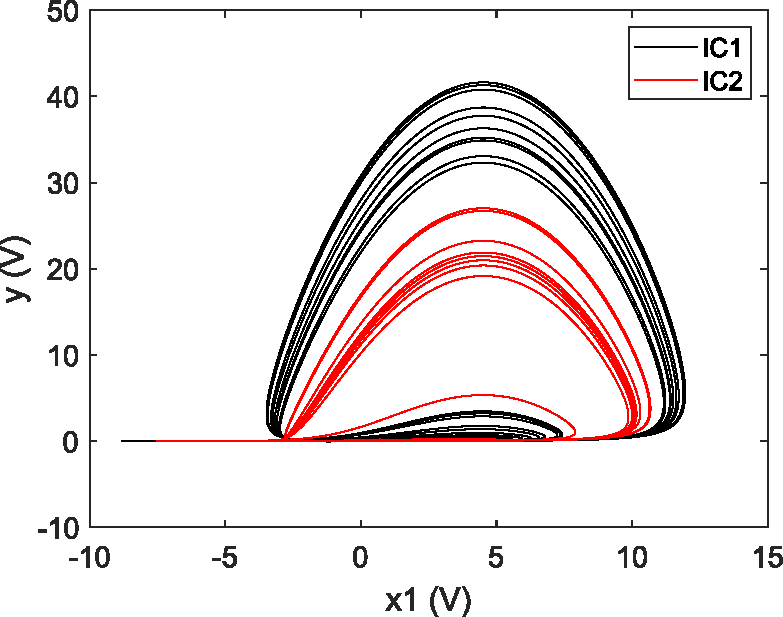
\includegraphics[scale=0.35]{figs/yvsx1Valid.pdf}
        \end{subfigure}
        \begin{subfigure}[b]{0.3\textwidth}  
            \centering 
            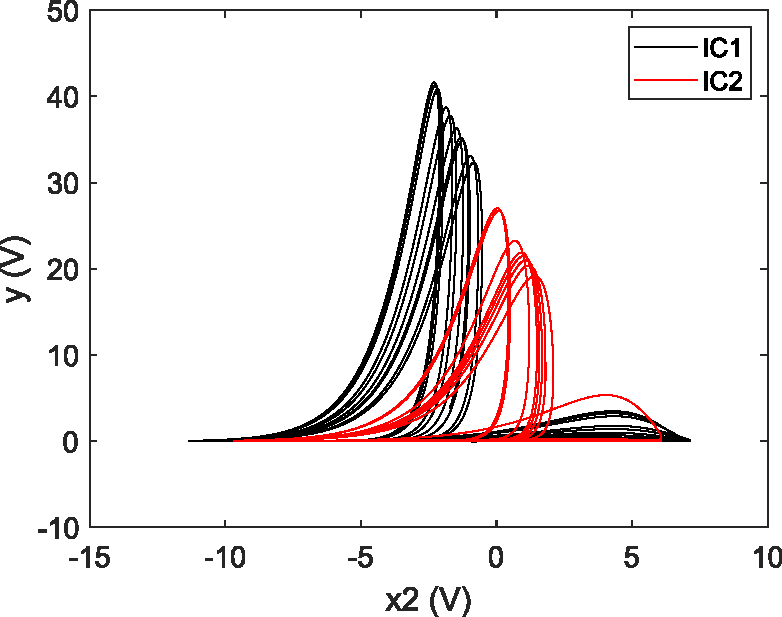
\includegraphics[scale=0.35]{figs/yvsx2Valid.pdf}
        \end{subfigure}
        \begin{subfigure}[b]{0.3\textwidth}   
            \centering 
            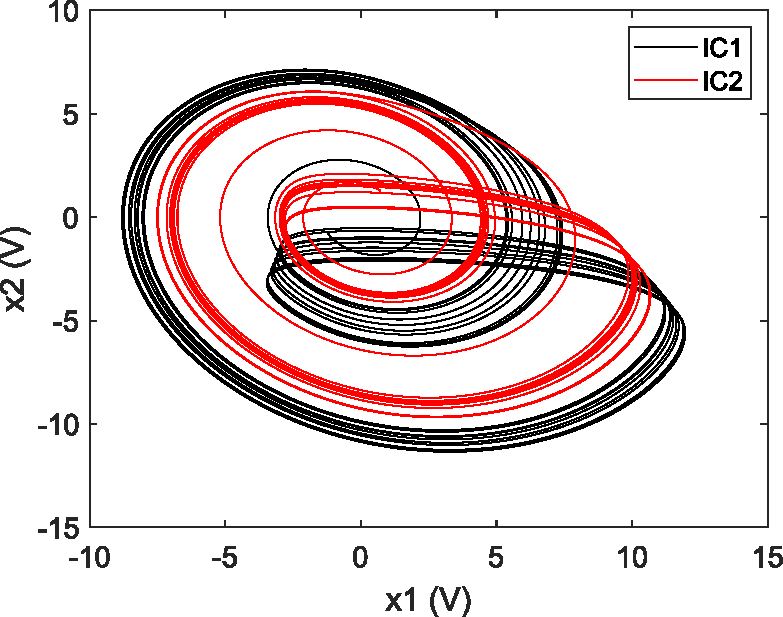
\includegraphics[scale=0.35]{figs/x2vsx1Valid.pdf}
        \end{subfigure}
        \caption{Phase portraits for the state variables with $IC1$ and $IC2$ as initial conditions.}
        \label{fig:validPhase}
	\end{figure*}

	\begin{figure*}
        \centering
        \begin{subfigure}[b]{0.3\textwidth}
            \centering
            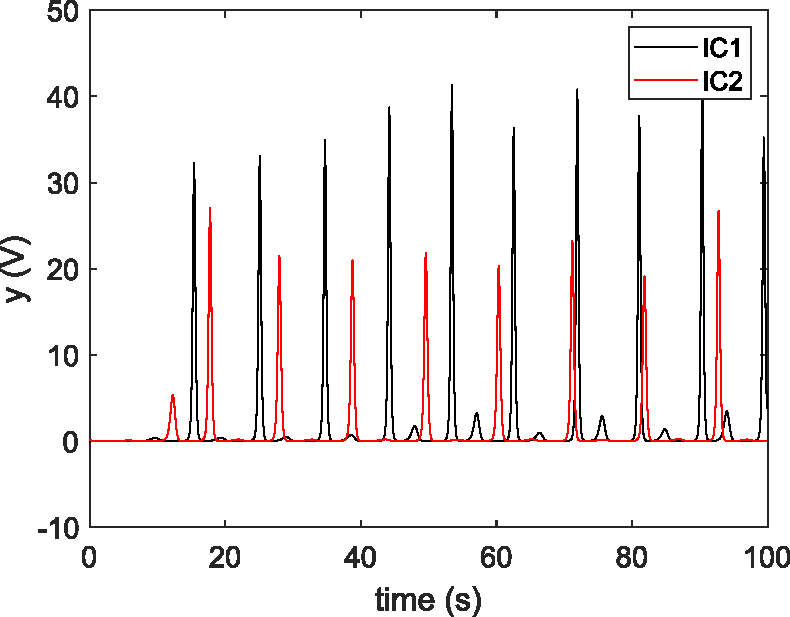
\includegraphics[scale=0.35]{figs/yvstValid.pdf}
        \end{subfigure}
        \begin{subfigure}[b]{0.3\textwidth}  
            \centering 
            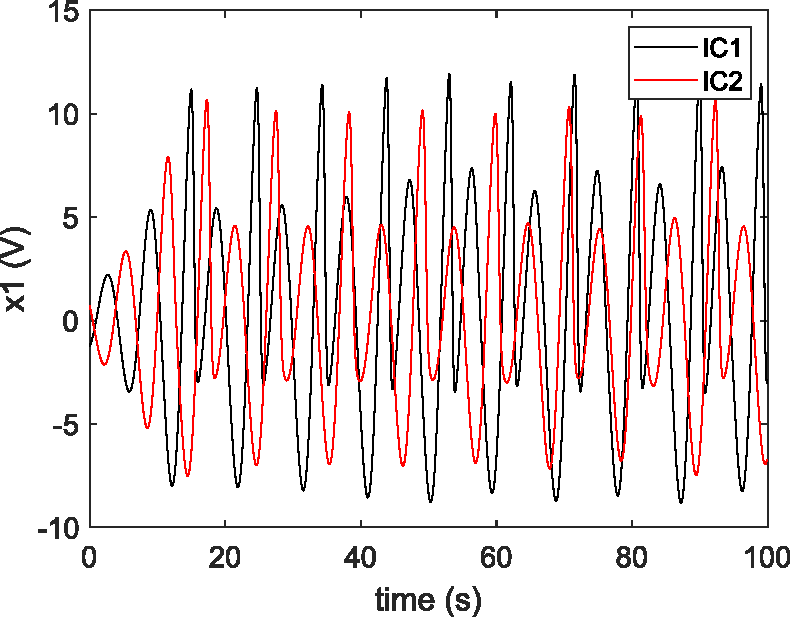
\includegraphics[scale=0.35]{figs/x1vstValid.pdf}
        \end{subfigure}
        \begin{subfigure}[b]{0.3\textwidth}   
            \centering 
            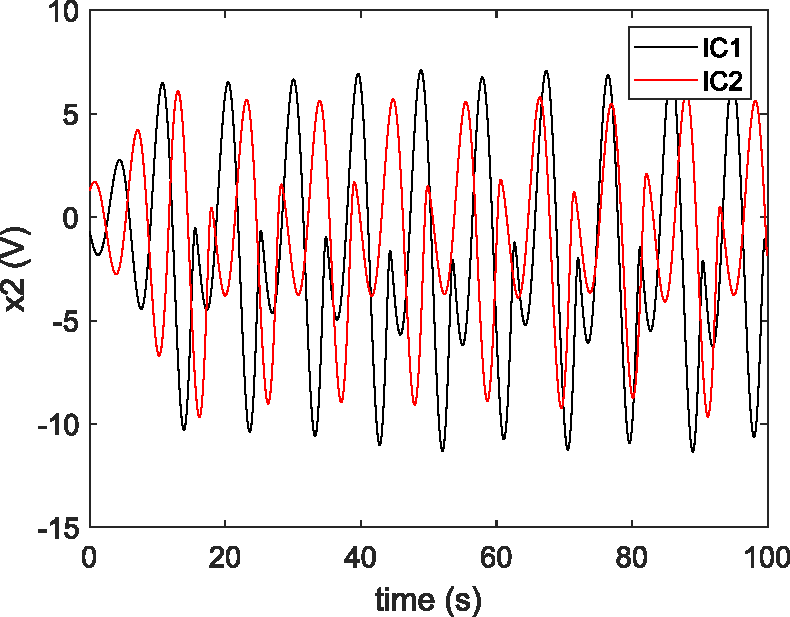
\includegraphics[scale=0.35]{figs/x2vstValid.pdf}
        \end{subfigure}
        \caption{Time responses for signals $y$, $x_1$, $x_2$ with initial conditions $IC1$ and $IC2$.}
        \label{fig:validTime}
	\end{figure*}
	%%%%%%%%%%%%%%%%%%%%%%%%%%%%%%%%%%%%%%%%%%%%%%%%%%%%%%%%%%%%%%%%%%%%%%%%%%%%%%
	\subsection{Input Variations}
	For comparing the results, we will be using the original R\"ossler model initialization \cite{rossler1976equation} as a reference and this simulation will be used for comparison. The parameters are $u(t)=0V$, $V_{cc0}=15V$, $RC=1s$, $R_a=500k\Omega$, $R_b=7500k\Omega$, $R_c=17.5439k\Omega$, with $t_0=0s$, $t_{\text{end}}=100s$ and initial conditions $(x_{10},x_{20},y_{0})=(0,-6.78,0.02)$. For all the following simulations, only the 3D plot for the state variables and the output response in time will be presented. In Figs. \ref{fig:3DRosslerO} and \ref{fig:RosslerO} the reference simulation results are presented. Three different inputs were selected according to our input definition: two sine waves and a step in the $V_{cc}$ voltage.
	
	\begin{figure}[H]
	    \centering
	    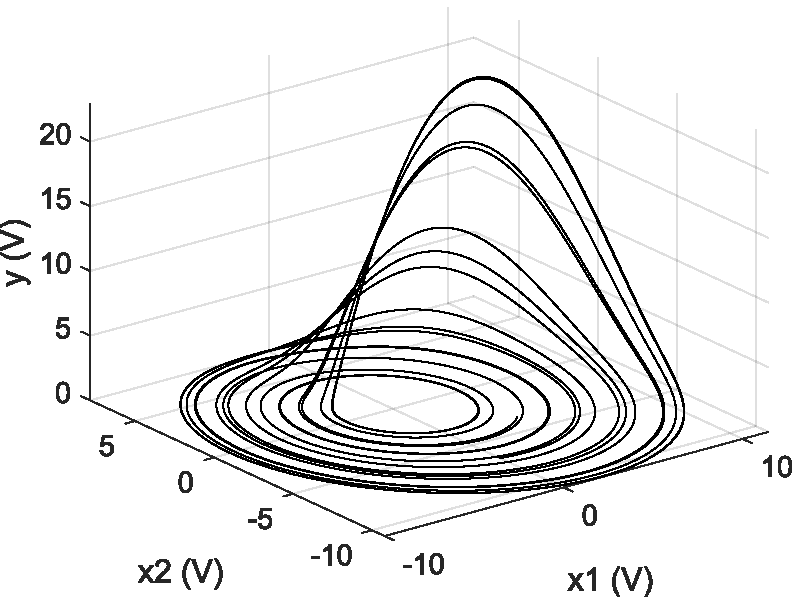
\includegraphics[scale=0.48]{figs/OriginalRosslerAttractor3d.pdf}
	    \caption{3D plot for the state variables and the output for reference Rössler attractor.}
	    \label{fig:3DRosslerO}
	\end{figure}
	\begin{figure}
	    \centering
	    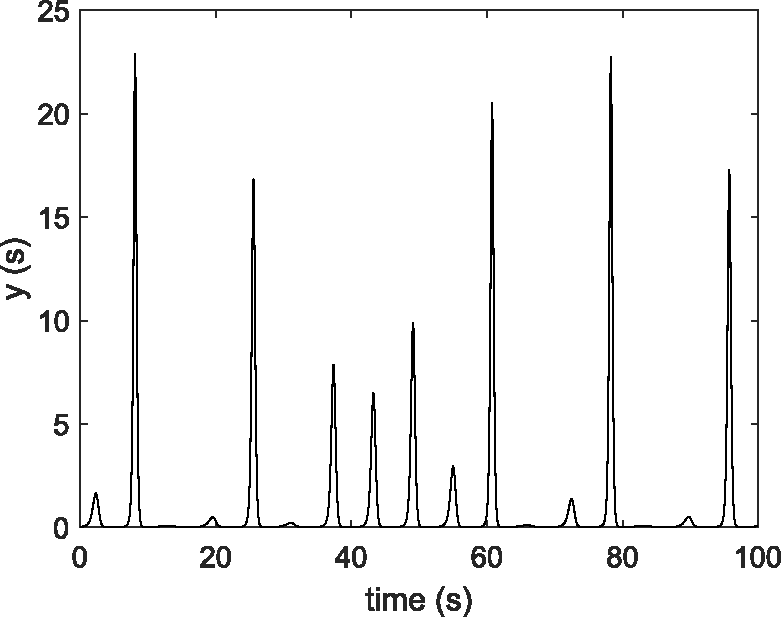
\includegraphics[scale=0.38]{figs/OriginalRosslery.pdf}
	    \caption{Output signal in time for reference Rössler attractor.}
	    \label{fig:RosslerO}
	\end{figure}
    It is important to highlight that the behavior showed in Fig. \ref{fig:RosslerO} is a good example of the response that Canals \textit{et al.} \cite{canals2014random} affirmed: the peaks in the output signal are unpredictable in time (this does not imply that the system is unpredictable).
	
    \subsubsection{Sines Inputs}\label{subsubsec:sines}
    First, a sine wave with frequency $\omega=2\text{rad}*s^{-1}$, amplitude $A=500V$ and offset of $b=500V$. Thus, the input is
    
    \begin{equation}
        u(t)=(500V)\sin({2t})+500V
    \end{equation}
    The plot for this input is shown in Fig. \ref{fig:inputSin2f}. The system's response is shown in Figs. \ref{fig:3dSin2f} and \ref{fig:OutSin2f}.
    \begin{figure}[H]
        \centering
        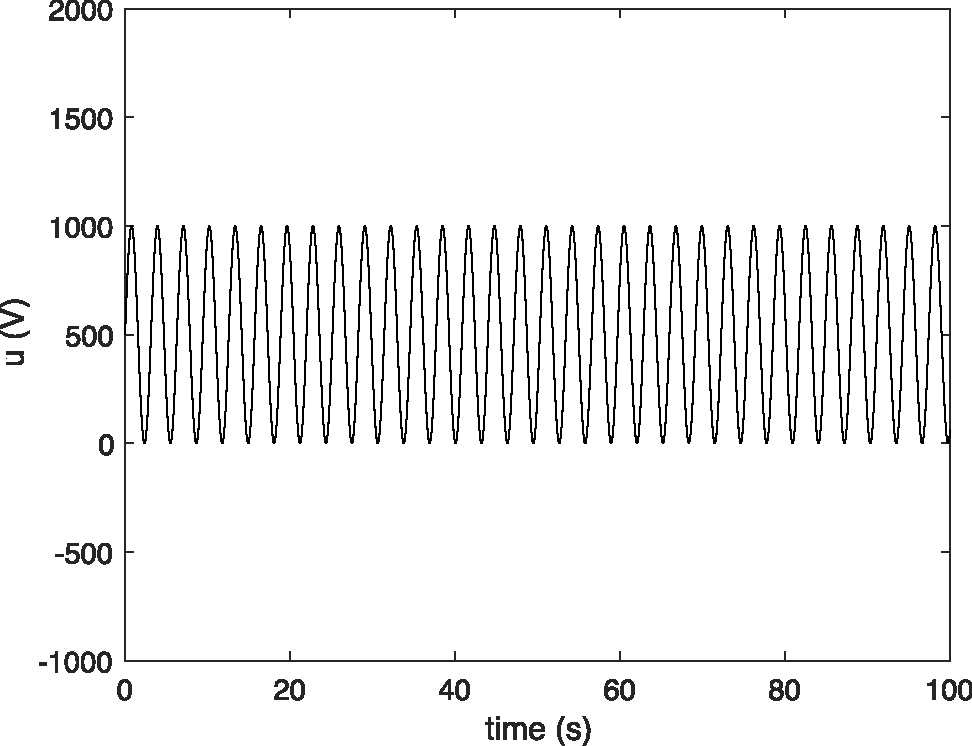
\includegraphics[scale=0.32]{figs/InputSin2f.pdf}
        \caption{Input sine wave with $\omega=2\text{rad}*s^{-1}$.}
        \label{fig:inputSin2f}
    \end{figure}
    \begin{figure}[H]
        \centering
        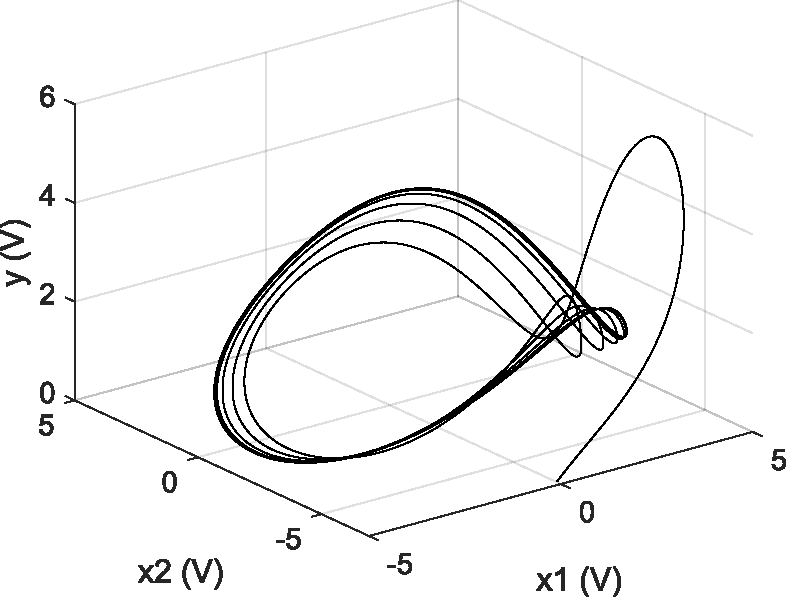
\includegraphics[scale=0.45]{figs/3dSine2fInput.pdf}
        \caption{Phase portrait for the three state variables with sine input.}
        \label{fig:3dSin2f}
    \end{figure}
    \begin{figure}[H]
        \centering
        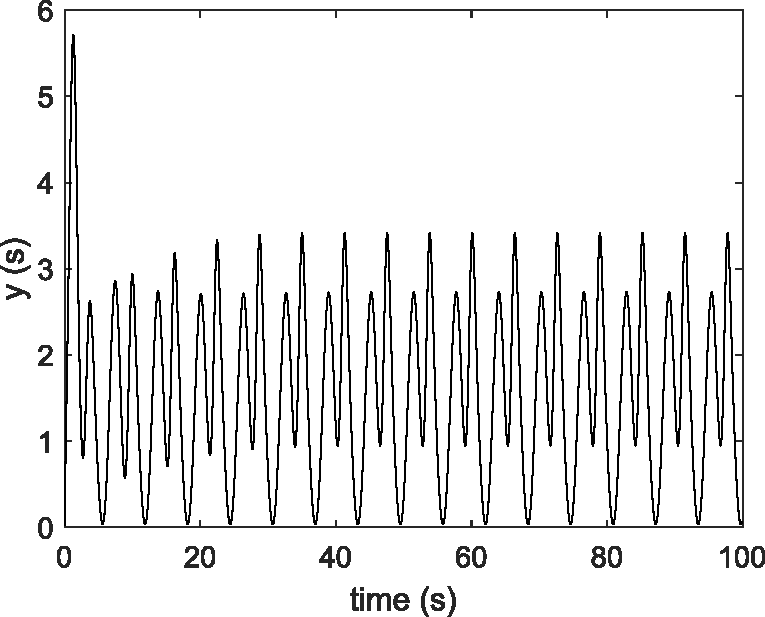
\includegraphics[scale=0.4]{figs/OutSine2fInput.pdf}
        \caption{Output signal response in time for sine input.}
        \label{fig:OutSin2f}
    \end{figure}
    
    Notice that eventually the trajectory falls in a closed and periodic orbit; as expected, the output signal is periodic but first modulated by an increasing signal.
    
    Second, a sine wave with frequency $\omega=5\text{rad}*s^{-1}$, amplitude $A=500V$ and offset of $b=500V$. Thus, the input is
    
    \begin{equation}
        u(t)=(500V)\sin({5t})+500V
    \end{equation}
    The plot for this input is shown in Fig. \ref{fig:inputSin5f}. The system's response is shown in Figs. \ref{fig:3dSin5f} and \ref{fig:OutSin5f}.
    
    \begin{figure}[H]
        \centering
        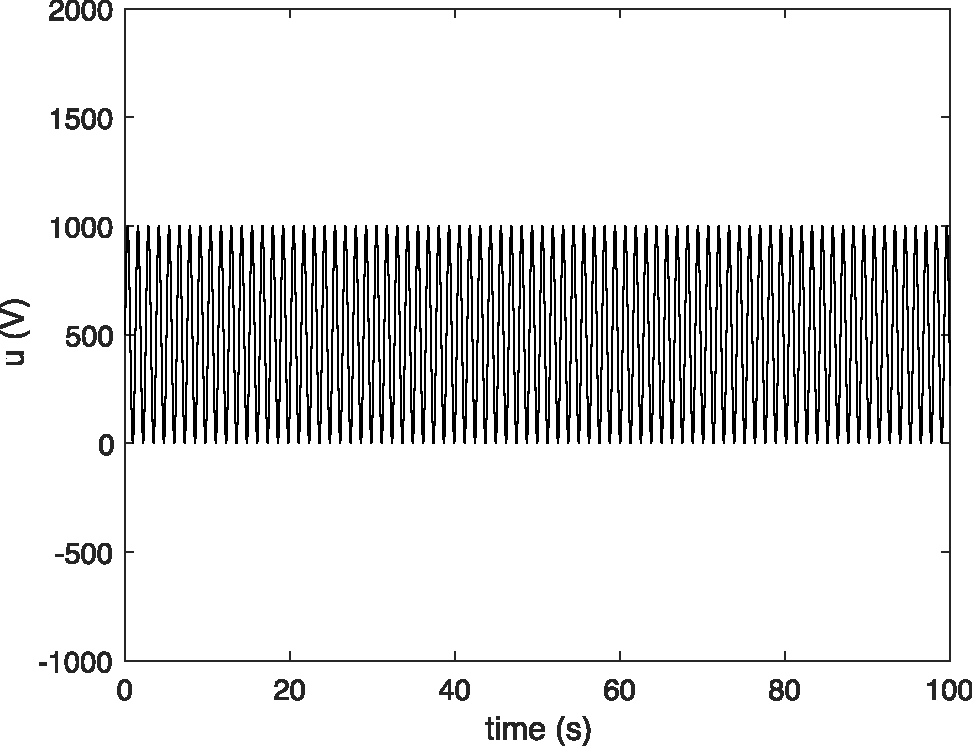
\includegraphics[scale=0.375]{figs/InputSin5f.pdf}
        \caption{Input sine wave with $\omega=5\text{rad}*s^{-1}$.}
        \label{fig:inputSin5f}
    \end{figure}
    \begin{figure}[H]
        \centering
        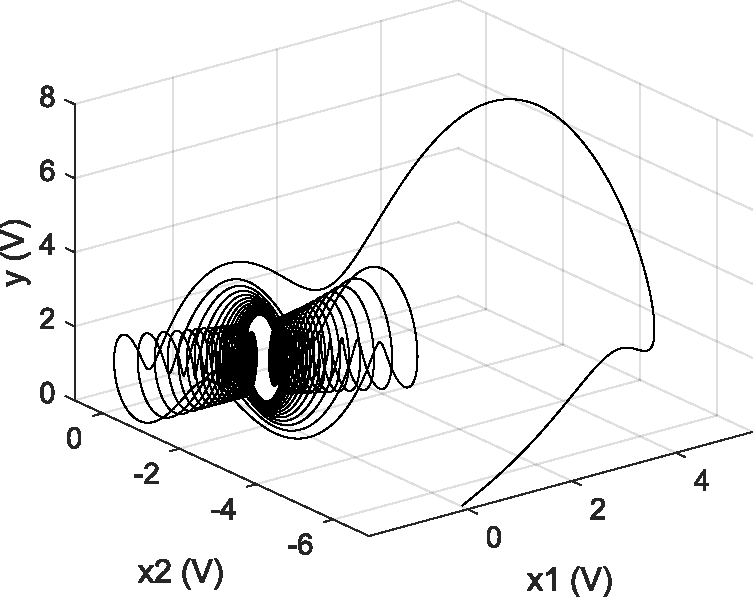
\includegraphics[scale=0.425]{figs/3dSine5fInput.pdf}
        \caption{Phase portrait for the three state variables with sine input.}
        \label{fig:3dSin5f}
    \end{figure}
    \begin{figure}[H]
        \centering
        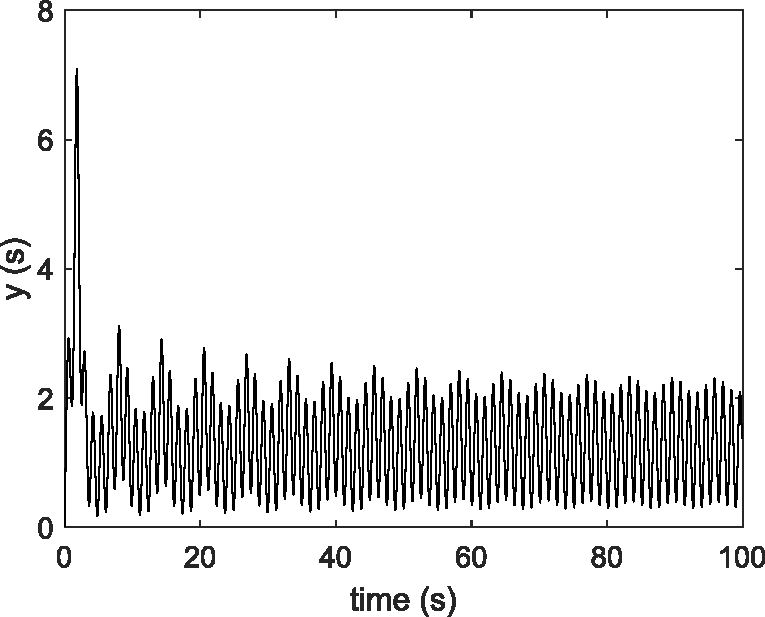
\includegraphics[scale=0.4]{figs/OutSine5fInput.pdf}
        \caption{Output signal response in time for sine input.}
        \label{fig:OutSin5f}
    \end{figure}
    
    As well as the previous sine input, the system falls into a periodic orbit that first decreases its amplitude. The output signal is periodic but modulated by a decreasing signal.
    
    \subsubsection{Step}\label{subsubsec:step}
    The step input was selected with step time of $40s$, initial value of $0V$ and final value of $1000V$. Hence, the input is given by
    
    \begin{equation}
        u(t)=(1000V)H(t-40s)
    \end{equation}
    Where $H(t)$ is the Heaviside step function. Fig. \ref{fig:inputStep} shows the step input and Figs. \ref{fig:3dStep} and \ref{fig:outStep} show the simulation results.
    \begin{figure}[H]
        \centering
        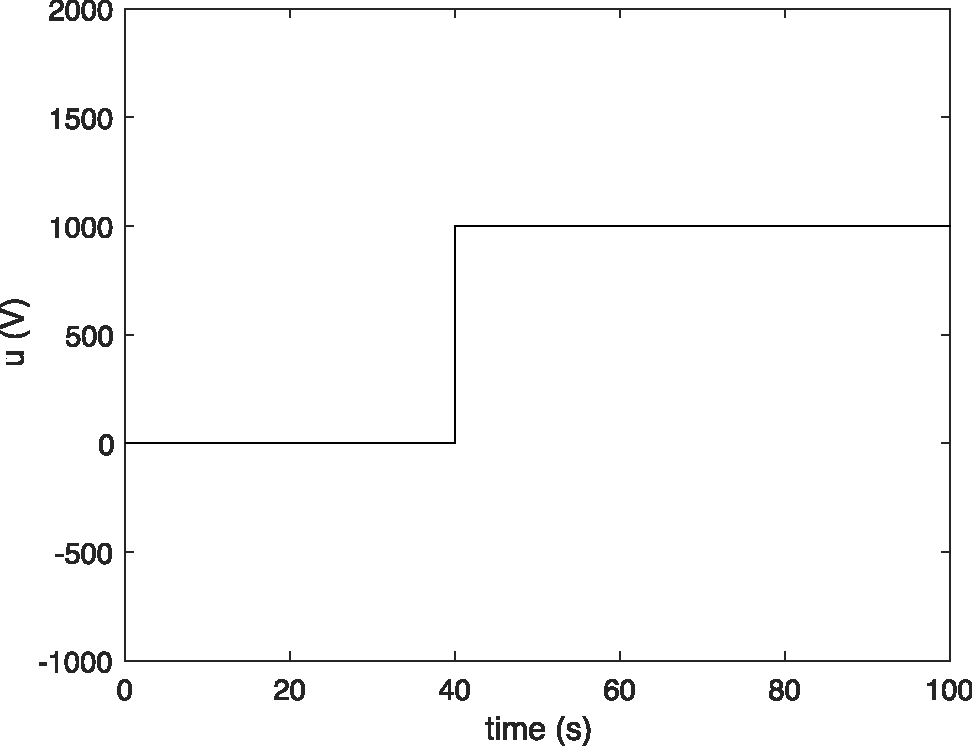
\includegraphics[scale=0.35]{figs/InputStep.pdf}
        \caption{Step input.}
        \label{fig:inputStep}
    \end{figure}
    \begin{figure}[H]
        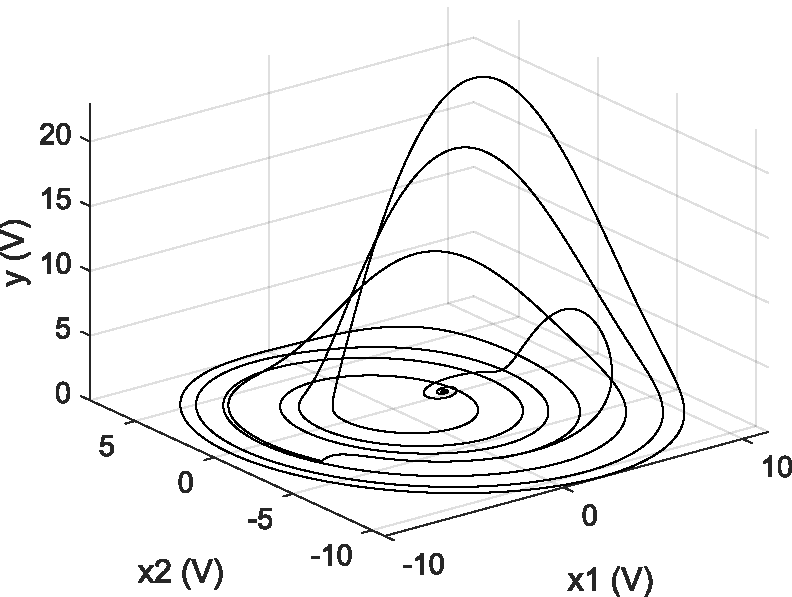
\includegraphics[scale=0.4]{figs/3dStepInput.pdf}
        \centering
        \caption{3D phase portrait for $x_1$, $x_2$ and $y$}
        \label{fig:3dStep}
    \end{figure}
    \begin{figure}[H]
        \centering
        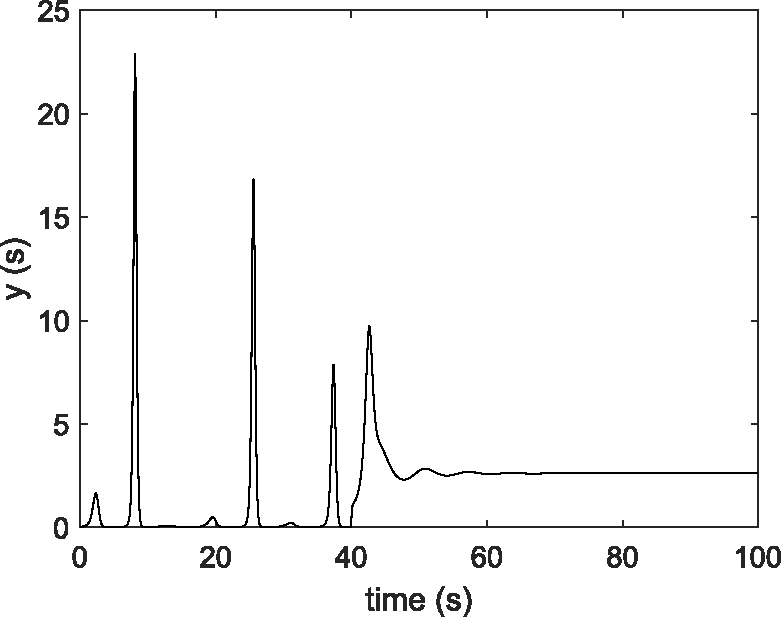
\includegraphics[scale=0.4]{figs/OutStepInput.pdf}
        \caption{Output signal response in time for step input.}
        \label{fig:outStep}
    \end{figure}
    
    The 3D plot for the state variables shows that it starts normally as the Rössler attractor, but once the input is applied, the system stabilizes in completely, converging to an specific point in space. In the output signal through time the stability is evidenced in the constant value for $y$. 
    
    %%%%%%%%%%%%%%%%%%%%%%%%%%%%%%%%%%%%%%%%%%%%%%%%%%%%%%%%%%%%%%%%%%%%%%%%%%%%%%
    \subsection{Parameter Variation}
    In this section, several simulations were made varying the values for parameters $R_a$ and $R_c$, choosing values with important impact in the system's response. All simulations were made assuming $u(t)=0V$, $V_{cc0}=15V$, $RC=1s$, $R_a=500k\Omega$, $R_b=7500k\Omega$, $R_c=17.5439k\Omega$, with $t_0=0s$, $t_{\text{end}}=100s$ and initial conditions $(x_{10},x_{20},y_{0})=(0,-6.78,0.02)$. Keep in mind that, when a parameter is selected to vary, the rest of the parameters, initial conditions and solution method remains the same.
    
    It is important to highlight that $R_b$ was not chosen for the parameter variation since varying it is similar to changing the input for the system.
    
    \subsubsection{Parameter \texorpdfstring{$R_a$}{Ra}}\label{subsubsec:varparaA}
    For parameter $R_a$, higher values from the reference $R_a=500k\Omega$ were selected, since smaller values than the reference produces behaviors similar enough with the reference system (Figs. \ref{fig:3DRosslerO} and \ref{fig:RosslerO}), even though there is a point where the response changes completely; this result will be presented in section \ref{subsubsec:ra}. The selected values for the parameter are $R_{a_1} = 650k\Omega$, $R_{a_2} = 750k\Omega$, $R_{a_3} = 1750k\Omega$ and $R_{a_4} = 3652k\Omega$. The results are shown in Figs. \ref{fig:3dparaAvar} and \ref{fig:paraAvar}.
    
    \begin{figure*}
        \centering
        \begin{subfigure}[b]{0.22\textwidth}
            \centering
            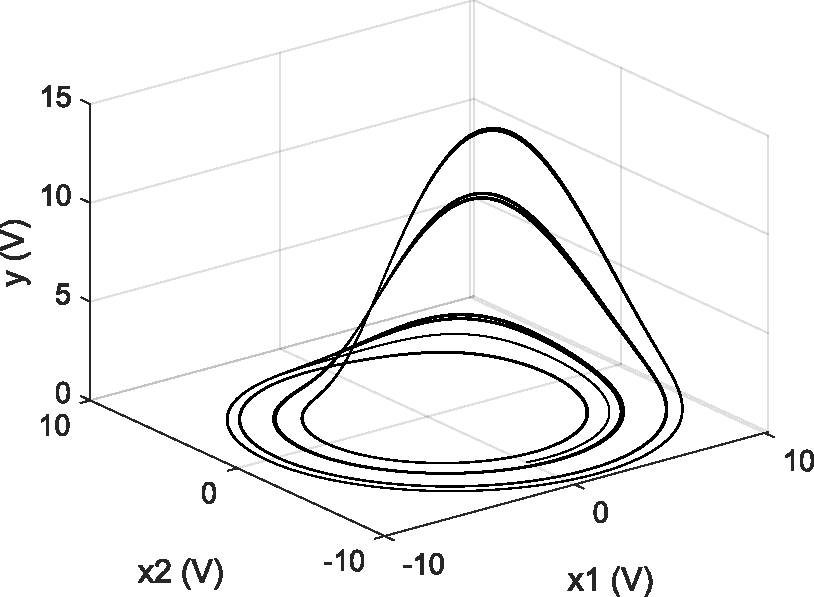
\includegraphics[scale=0.28]{figs/paraA/3dParaA650.pdf}
            \caption{$R_{a_1} = 650k\Omega$.}    
        \end{subfigure}
        \begin{subfigure}[b]{0.22\textwidth}  
            \centering 
            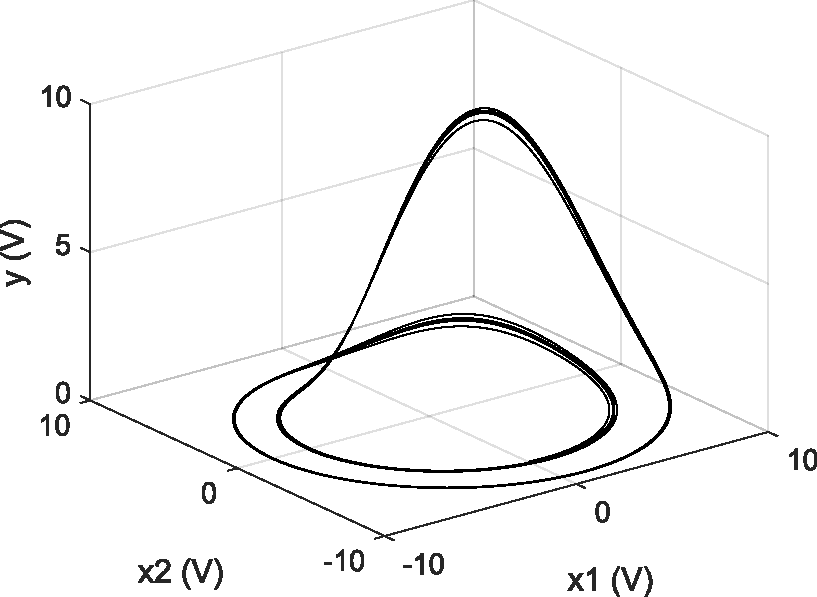
\includegraphics[scale=0.28]{figs/paraA/3dParaA750.pdf}
            \caption{$R_{a_2} = 750k\Omega$.}  
        \end{subfigure}
        \begin{subfigure}[b]{0.22\textwidth}   
            \centering 
            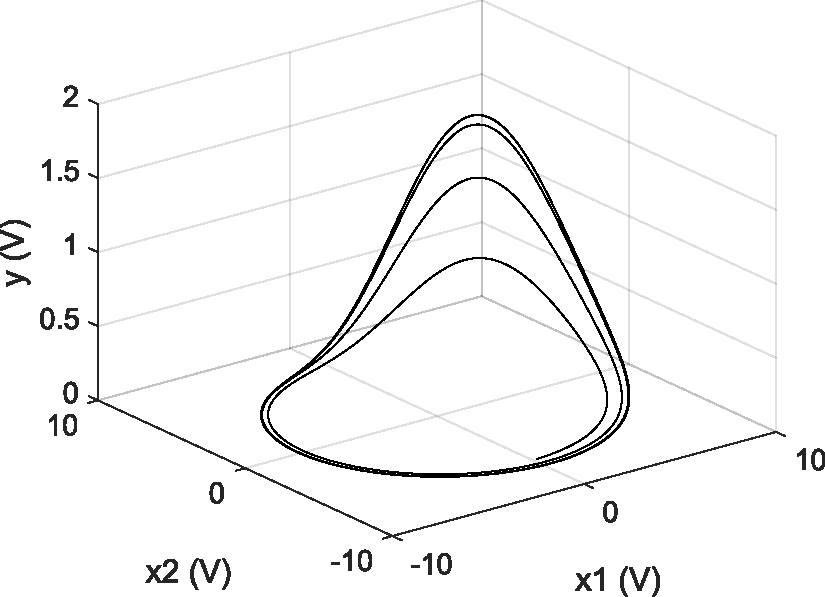
\includegraphics[scale=0.28]{figs/paraA/3dParaA1750.pdf}
            \caption{$R_{a_3} = 1750k\Omega$}    
        \end{subfigure}
        \begin{subfigure}[b]{0.22\textwidth}   
            \centering 
            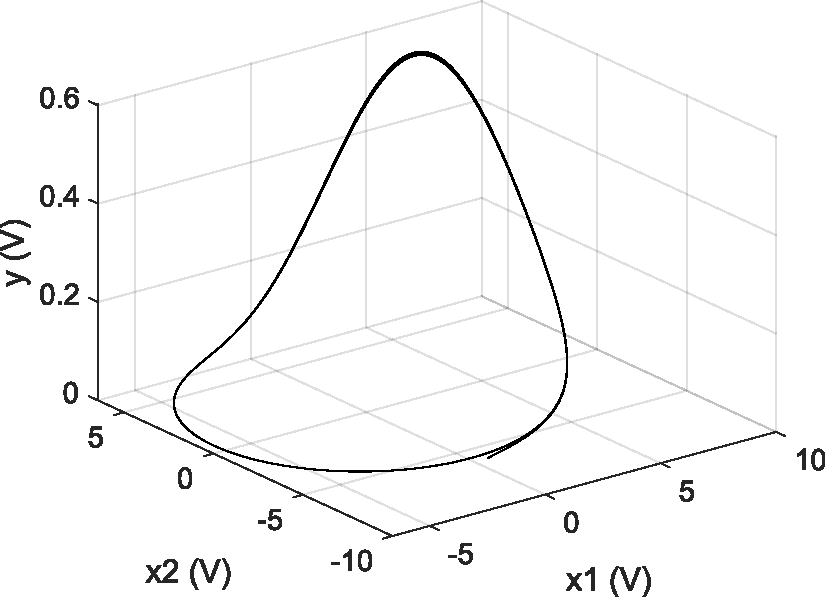
\includegraphics[scale=0.28]{figs/paraA/3dParaA3652.pdf}
            \caption{$R_{a_4} = 3652k\Omega$}   
            \label{fig:3dparaAvard}
        \end{subfigure}
        \caption{3D results for increments in $R_a$.} 
        \label{fig:3dparaAvar}
	\end{figure*}
	
	    \begin{figure*}
        \centering
        \begin{subfigure}[b]{0.22\textwidth}
            \centering
            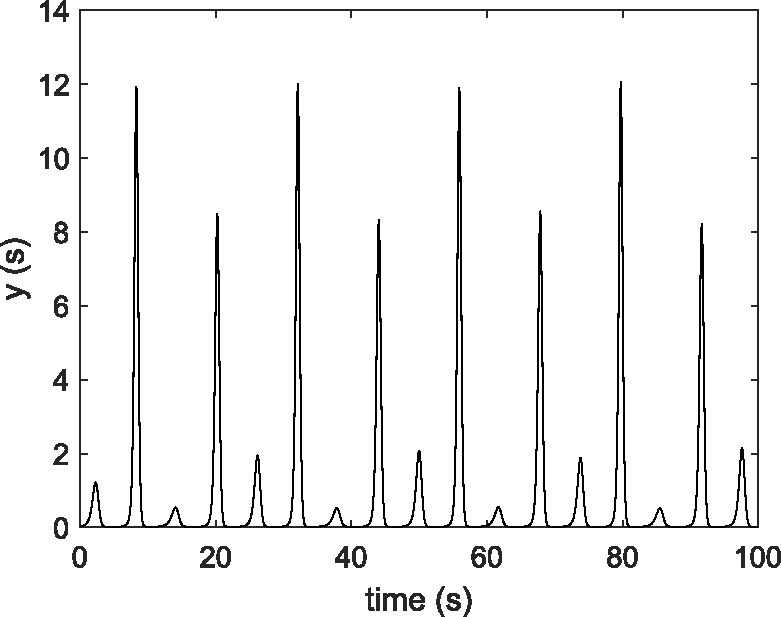
\includegraphics[scale=0.28]{figs/paraA/outParaA650.pdf}
            \caption{$R_{a_1} = 650k\Omega$.}    
        \end{subfigure}
        \begin{subfigure}[b]{0.22\textwidth}  
            \centering 
            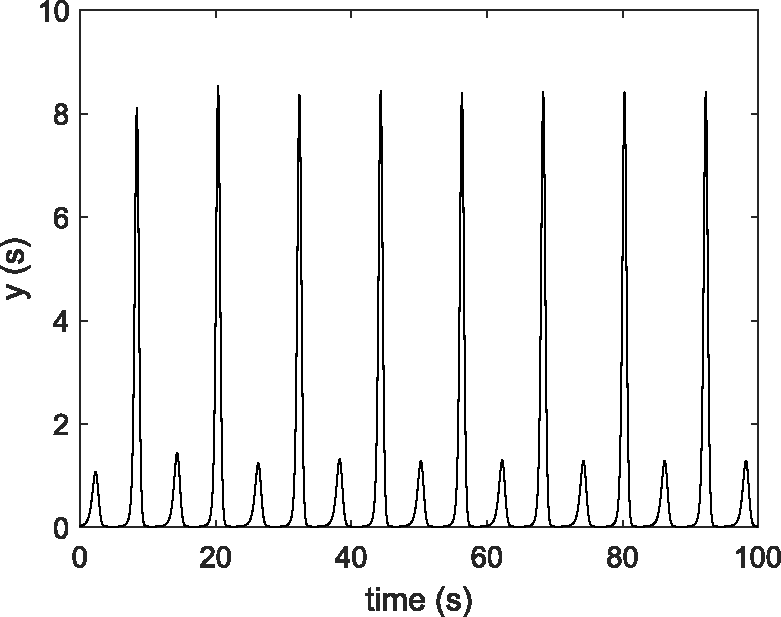
\includegraphics[scale=0.28]{figs/paraA/outParaA750.pdf}
            \caption{$R_{a_2} = 750k\Omega$.}  
        \end{subfigure}
        \begin{subfigure}[b]{0.22\textwidth}   
            \centering 
            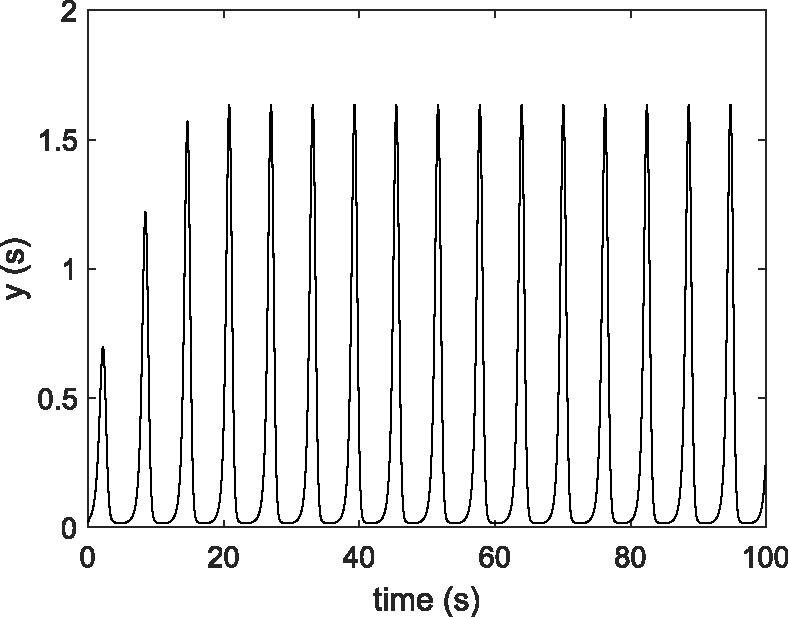
\includegraphics[scale=0.28]{figs/paraA/outParaA1750.pdf}
            \caption{$R_{a_3} = 1750k\Omega$}    
        \end{subfigure}
        \begin{subfigure}[b]{0.22\textwidth}   
            \centering 
            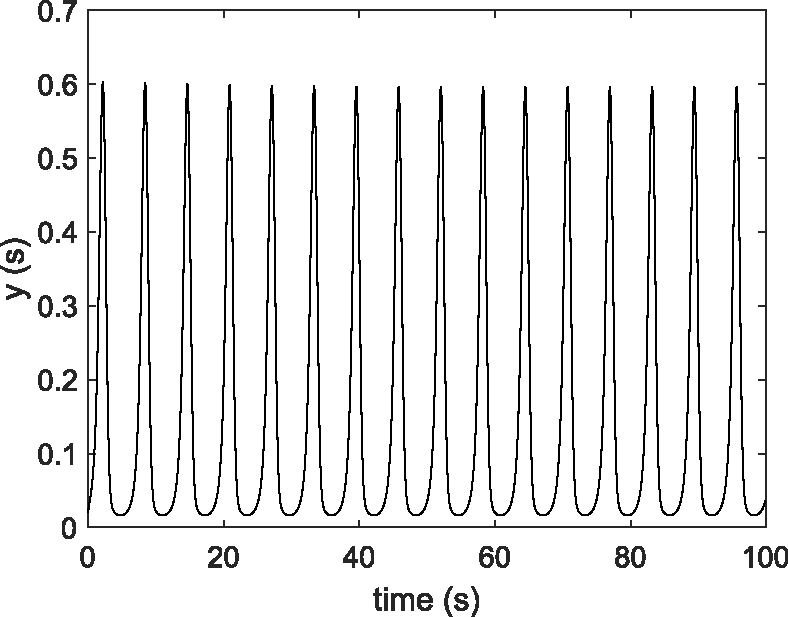
\includegraphics[scale=0.28]{figs/paraA/outParaA3652.pdf}
            \caption{$R_{a_4} = 3652k\Omega$}   
        \end{subfigure}
        \caption{Output signal in time for increments in $R_a$} 
        \label{fig:paraAvar}
	\end{figure*}
    
    \subsubsection{Parameter \texorpdfstring{$R_c$}{Rc}}\label{subsubsec:varparaC}
    Following the procedure of the previous section, both increments and smaller values of $R_c$ have been selected to evidence the response of the system. For the smaller values $R_{c_1}=10k\Omega$, $R_{c_2}=5k\Omega$, $R_{c_3}=2k\Omega$ and $R_{c_4}=1k\Omega$ have been selected. The results for the simulations with this parameters are shown in Figs. \ref{fig:3dparaCvarDown} and \ref{fig:paraCvarDown}.
    \begin{figure*}
        \centering
        \begin{subfigure}[b]{0.22\textwidth}
            \centering
            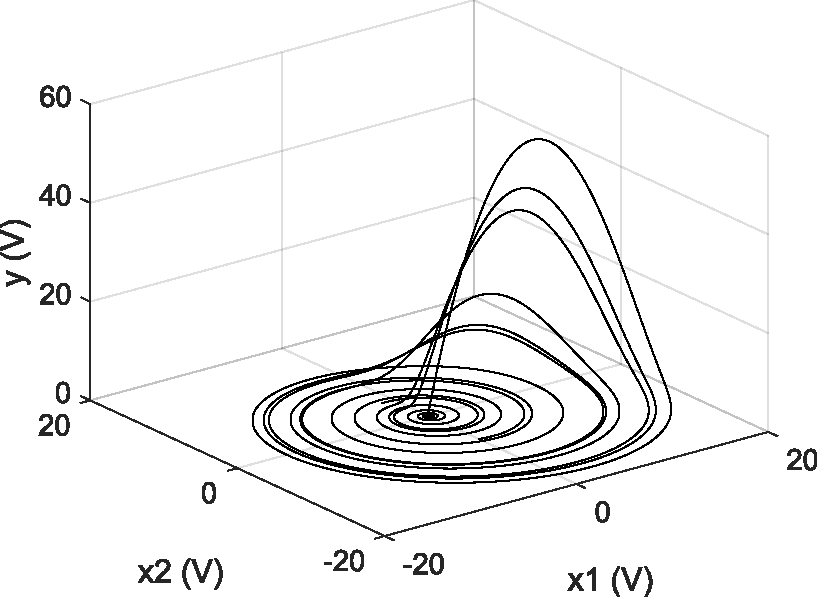
\includegraphics[scale=0.28]{figs/paraCdown/3dParaC10.pdf}
            \caption{$R_{c_1} = 10k\Omega$.}    
        \end{subfigure}
        \begin{subfigure}[b]{0.22\textwidth}  
            \centering 
            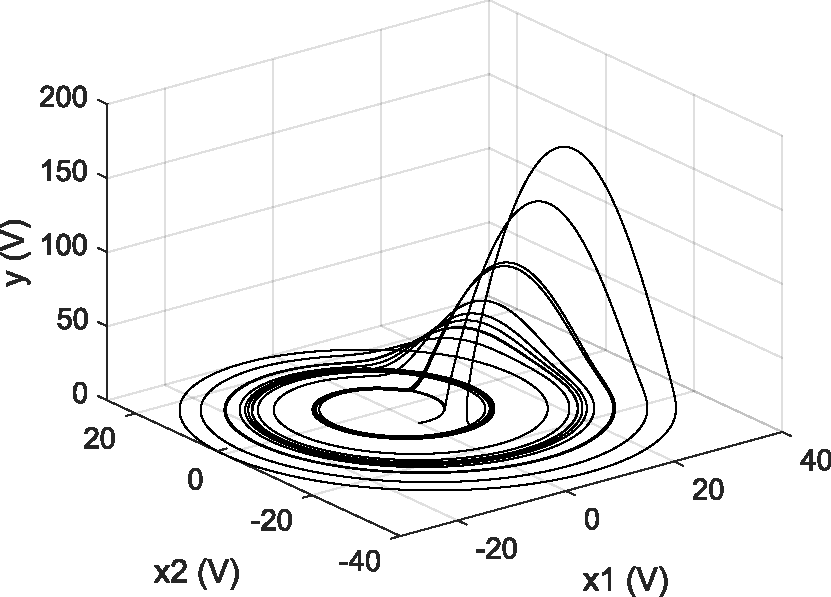
\includegraphics[scale=0.28]{figs/paraCdown/3dParaC5.pdf}
            \caption{$R_{c_2} = 5k\Omega$.}  
        \end{subfigure}
        \begin{subfigure}[b]{0.22\textwidth}   
            \centering 
            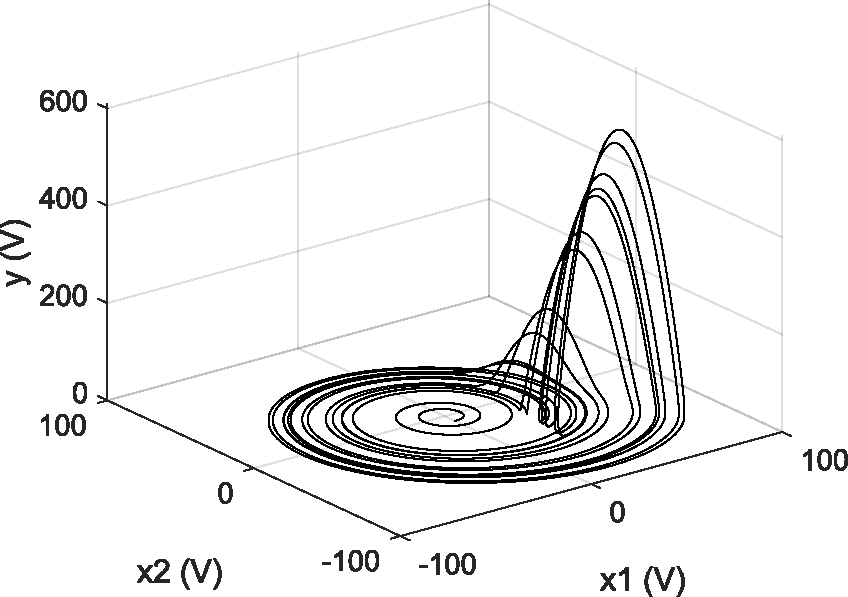
\includegraphics[scale=0.28]{figs/paraCdown/3dParaC2.pdf}
            \caption{$R_{c_3} = 2k\Omega$}    
        \end{subfigure}
        \begin{subfigure}[b]{0.22\textwidth}   
            \centering 
            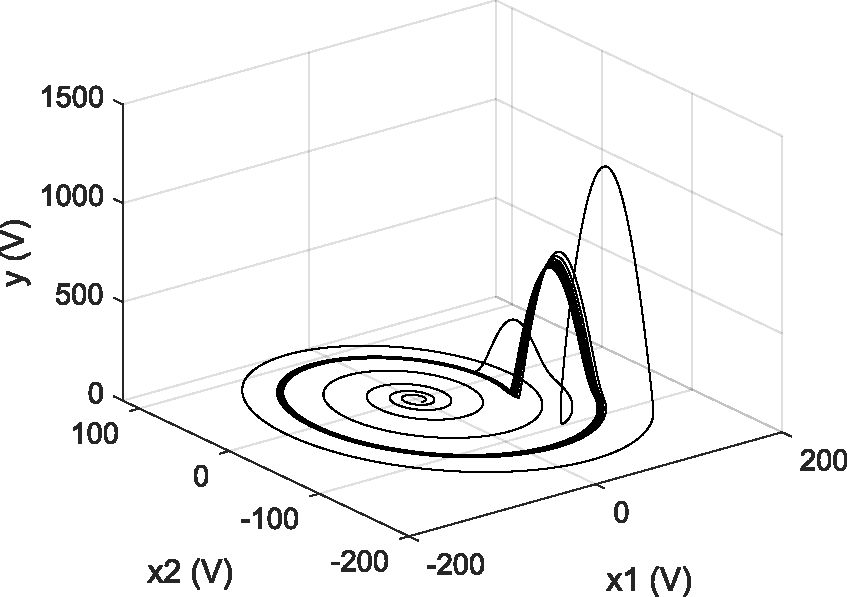
\includegraphics[scale=0.28]{figs/paraCdown/3dParaC1.pdf}
            \caption{$R_{c_4} = 1k\Omega$}
        \end{subfigure}
        \caption{3D results for smaller values of $R_c$.} 
        \label{fig:3dparaCvarDown}
	\end{figure*}
	
	    \begin{figure*}
        \centering
        \begin{subfigure}[b]{0.22\textwidth}
            \centering
            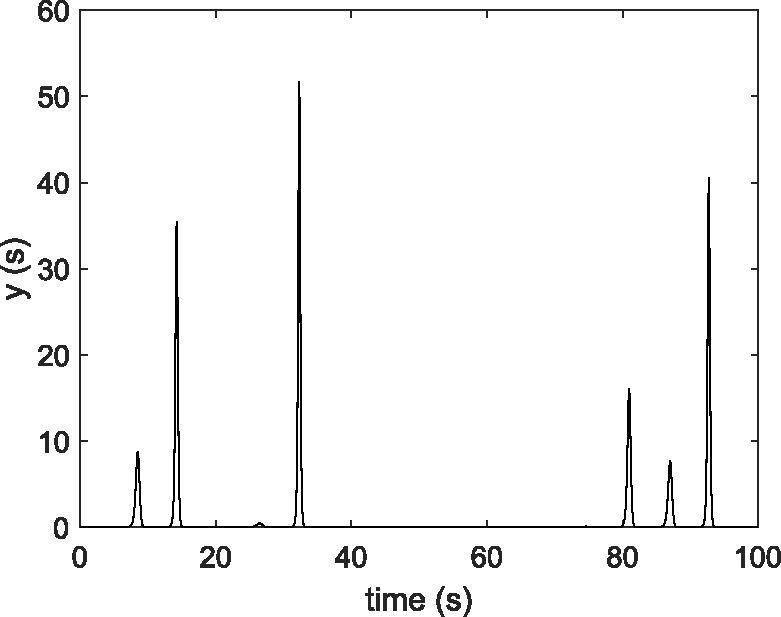
\includegraphics[scale=0.28]{figs/paraCdown/outParaC10.pdf}
            \caption{$R_{c_1} = 10k\Omega$.}    
        \end{subfigure}
        \begin{subfigure}[b]{0.22\textwidth}  
            \centering 
            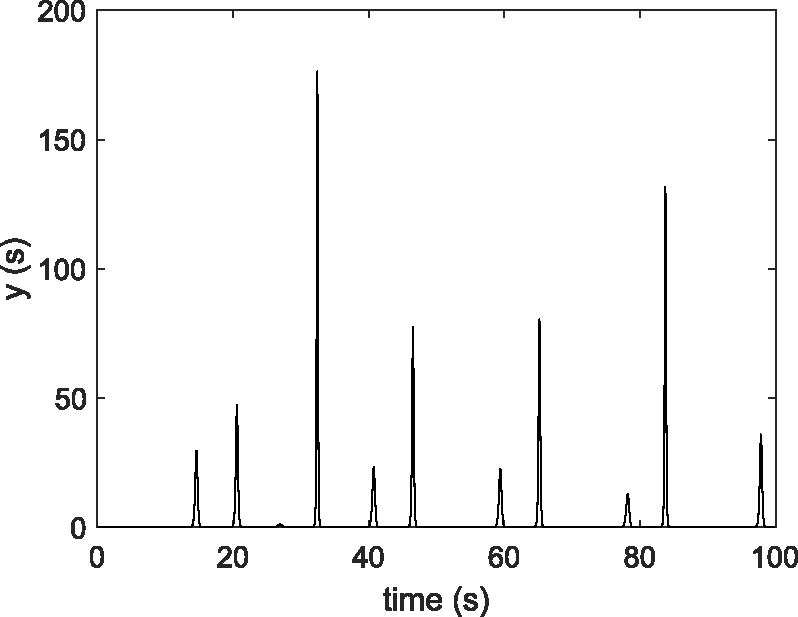
\includegraphics[scale=0.28]{figs/paraCdown/outParaC5.pdf}
            \caption{$R_{c_2} = 5k\Omega$.}  
        \end{subfigure}
        \begin{subfigure}[b]{0.22\textwidth}
            \centering 
            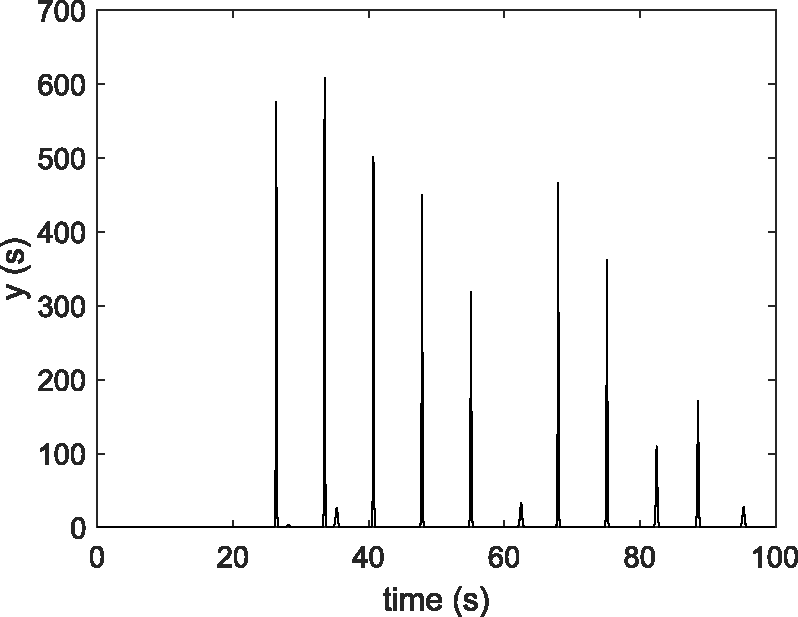
\includegraphics[scale=0.28]{figs/paraCdown/outParaC2.pdf}
            \caption{$R_{c_3} = 2k\Omega$}    
        \end{subfigure}
        \begin{subfigure}[b]{0.22\textwidth}   
            \centering 
            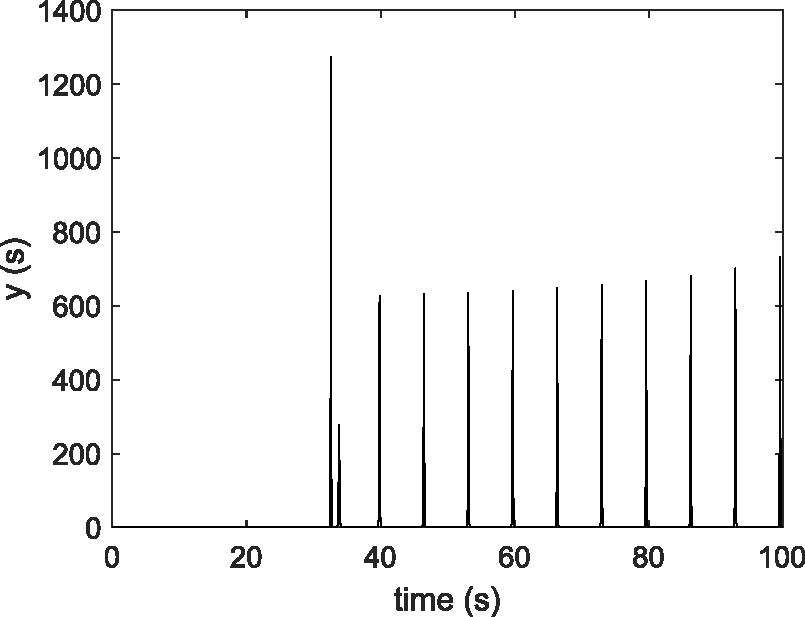
\includegraphics[scale=0.28]{figs/paraCdown/outParaC1.pdf}
            \caption{$R_{c_4} = 1k\Omega$}   
        \end{subfigure}
        \caption{Output signal in time for smaller values of $R_c$} 
        \label{fig:paraCvarDown}
	\end{figure*}
	
	For greater values, $R_{c_5}=10k\Omega$, $R_{c_6}=5k\Omega$, $R_{c_7}=2k\Omega$ and $R_{c_8}=1k\Omega$ were selected. The simulation results are shown in Figs. \ref{fig:3dparaCvarUp} and \ref{fig:paraCvarUp}.
	
	\begin{figure*}
        \centering
        \begin{subfigure}[b]{0.22\textwidth}
            \centering
            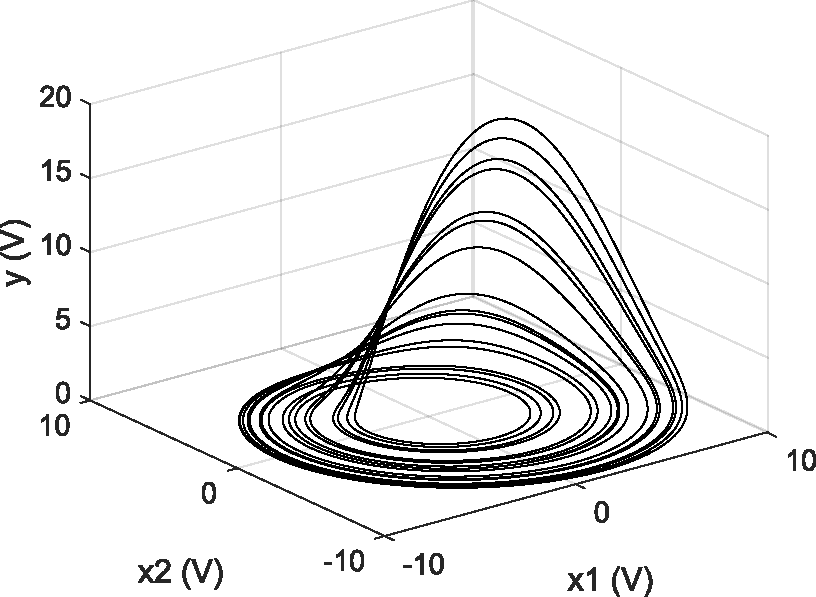
\includegraphics[scale=0.28]{figs/paraCup/3dParaC20.pdf}
            \caption{$R_{c_5} = 20k\Omega$.}    
        \end{subfigure}
        \begin{subfigure}[b]{0.22\textwidth}  
            \centering 
            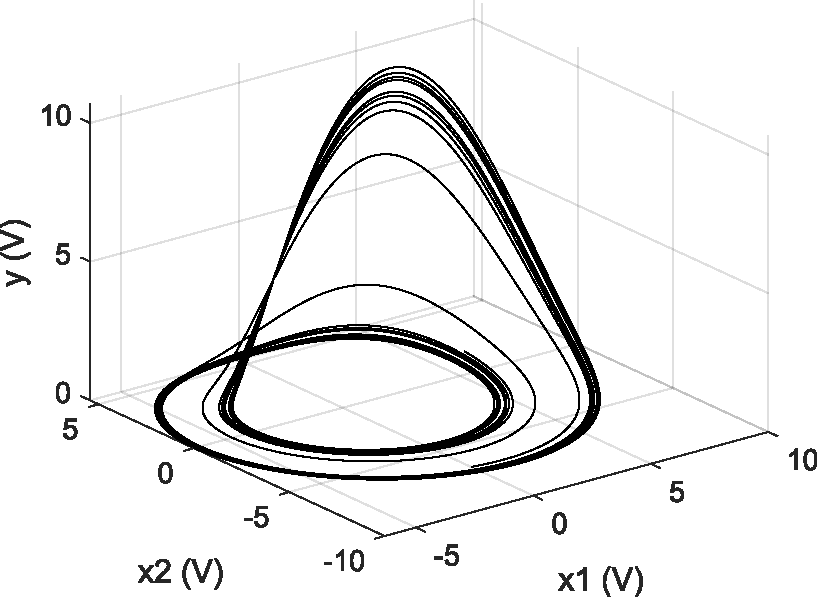
\includegraphics[scale=0.28]{figs/paraCup/3dParaC25.pdf}
            \caption{$R_{c_7} = 25k\Omega$.}  
        \end{subfigure}
        \begin{subfigure}[b]{0.22\textwidth}   
            \centering 
            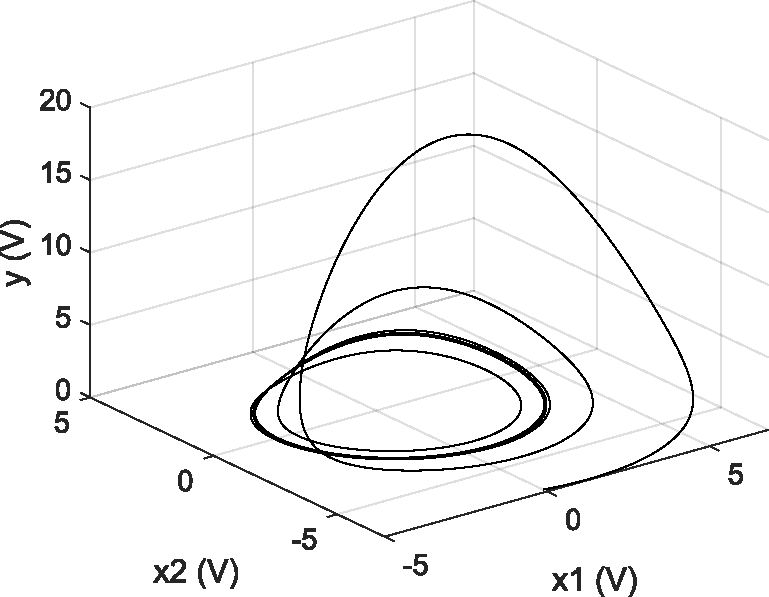
\includegraphics[scale=0.28]{figs/paraCup/3dParaC50.pdf}
            \caption{$R_{c_7} = 50k\Omega$}    
        \end{subfigure}
        \begin{subfigure}[b]{0.22\textwidth}   
            \centering 
            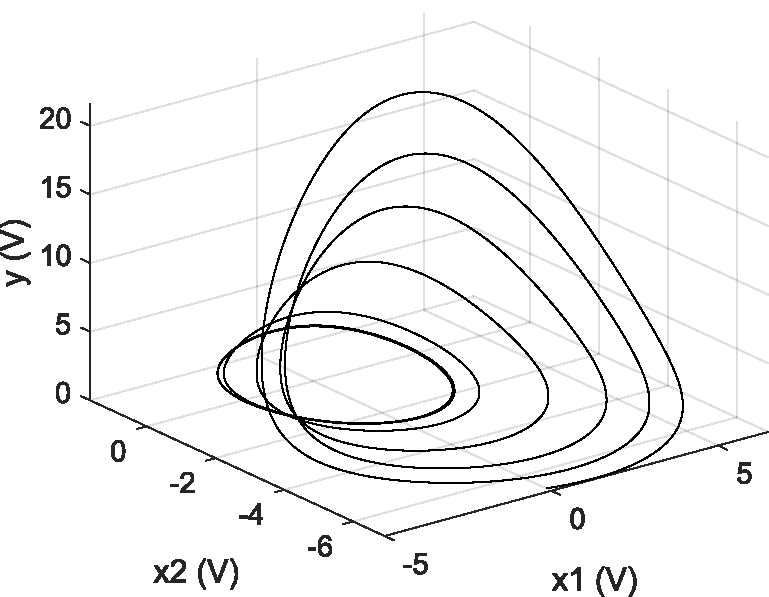
\includegraphics[scale=0.28]{figs/paraCup/3dParaC75.pdf}
            \caption{$R_{c_8} = 75k\Omega$}   
        \end{subfigure}
        \caption{3D results for increments in $R_c$.} 
        \label{fig:3dparaCvarUp}
	\end{figure*}
	
	    \begin{figure*}
        \centering
        \begin{subfigure}[b]{0.22\textwidth}
            \centering
            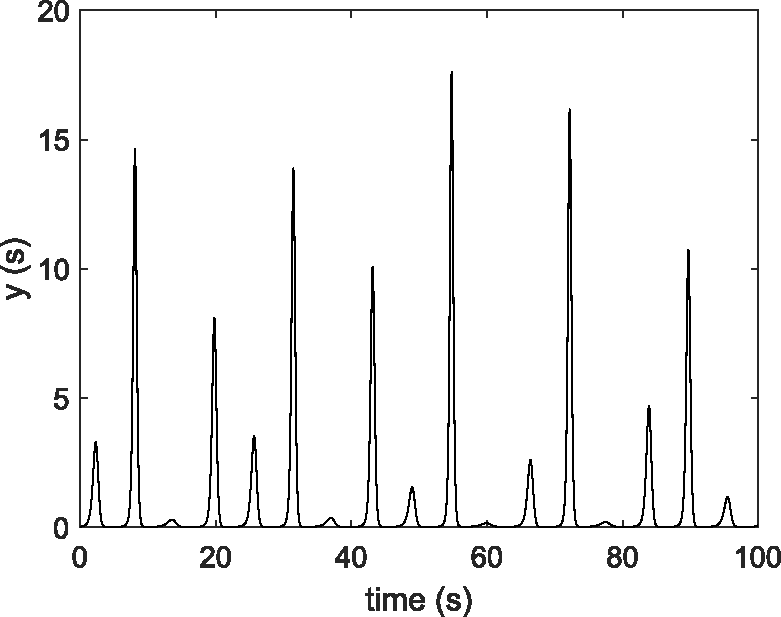
\includegraphics[scale=0.28]{figs/paraCup/outParaC20.pdf}
            \caption{$R_{c_5} = 20k\Omega$.}    
        \end{subfigure}
        \begin{subfigure}[b]{0.22\textwidth}  
            \centering 
            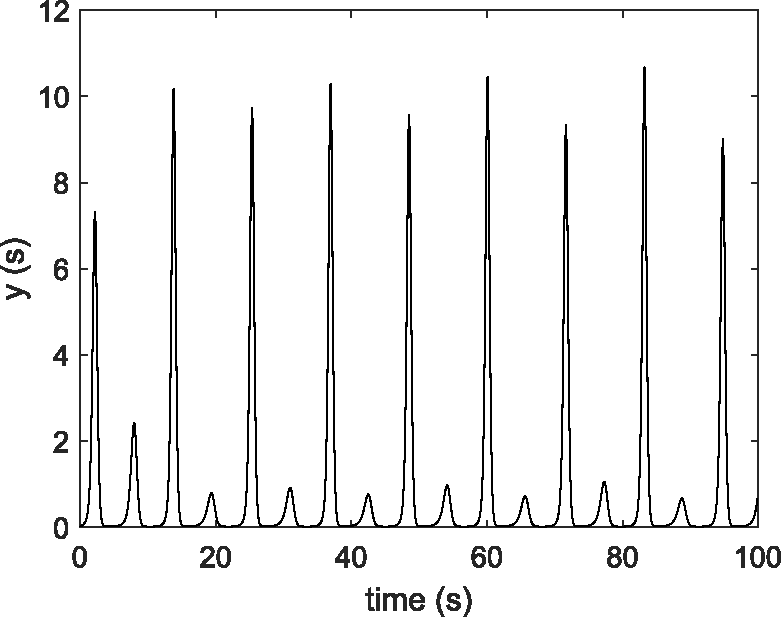
\includegraphics[scale=0.28]{figs/paraCup/outParaC25.pdf}
            \caption{$R_{c_6} = 25k\Omega$.}  
        \end{subfigure}
        \begin{subfigure}[b]{0.22\textwidth}   
            \centering 
            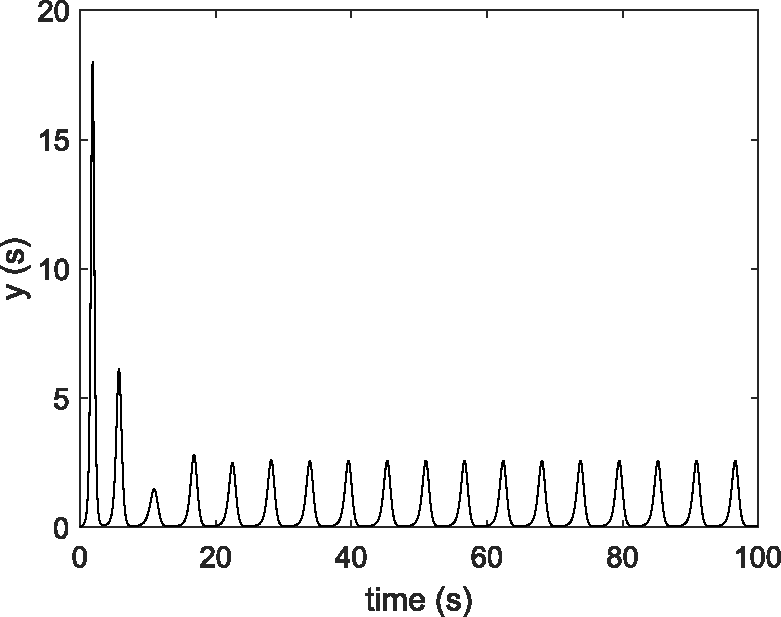
\includegraphics[scale=0.28]{figs/paraCup/outParaC50.pdf}
            \caption{$R_{c_7} = 50k\Omega$}    
        \end{subfigure}
        \begin{subfigure}[b]{0.22\textwidth}
            \centering 
            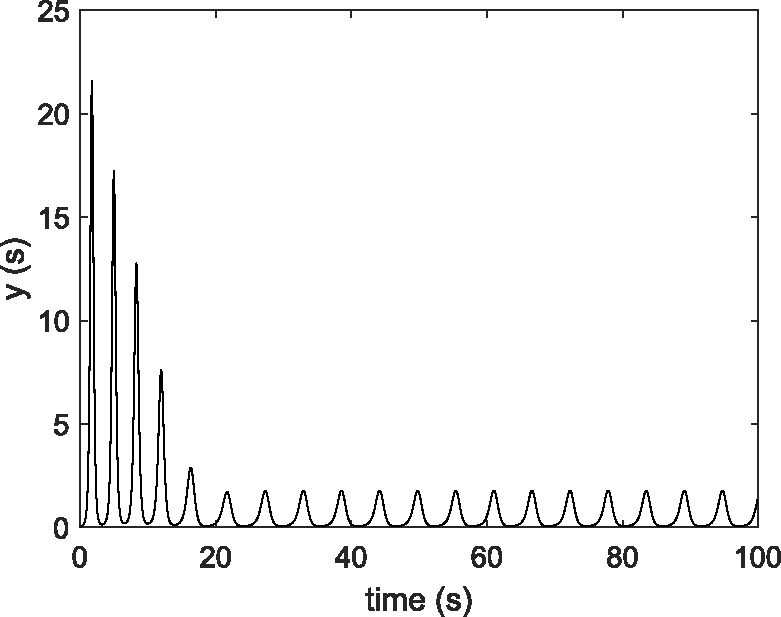
\includegraphics[scale=0.28]{figs/paraCup/outParaC75.pdf}
            \caption{$R_{c_8} = 75k\Omega$}  
            \label{fig:paraCvarUpd}
        \end{subfigure}
        \caption{Output signal in time for increments in $R_c$} 
        \label{fig:paraCvarUp}
	\end{figure*}
	
    %%%%%%%%%%%%%%%%%%%%%%%%%%%%%%%%%%%%%%%%%%%%%%%%%%%%%%%%%%%%%%%%%%%%%%%%%%%%%%
    \subsection{Limit for Parameter Variation}
    In the following simulations, extreme values for $R_a$ and $R_c$ are presented; that is, values for which the output $y$ starts to behave unaccordigly. The values presented here were found following a bisection method, between a known normal behavior for the system and a point where the derivative in the simulation was not finite.
    
    \subsubsection{Parameter \texorpdfstring{$R_a$}{Ra}}\label{subsubsec:ra}
    First, a significantly close value to the minimum for $R_a$ was obtained around $259.098131084k\Omega$. In Figs. \ref{fig:outParaAdown} and \ref{fig:3dParaAdown} the behavior of the output in time and all three variables is shown.
    \begin{figure}[H]
        \centering
        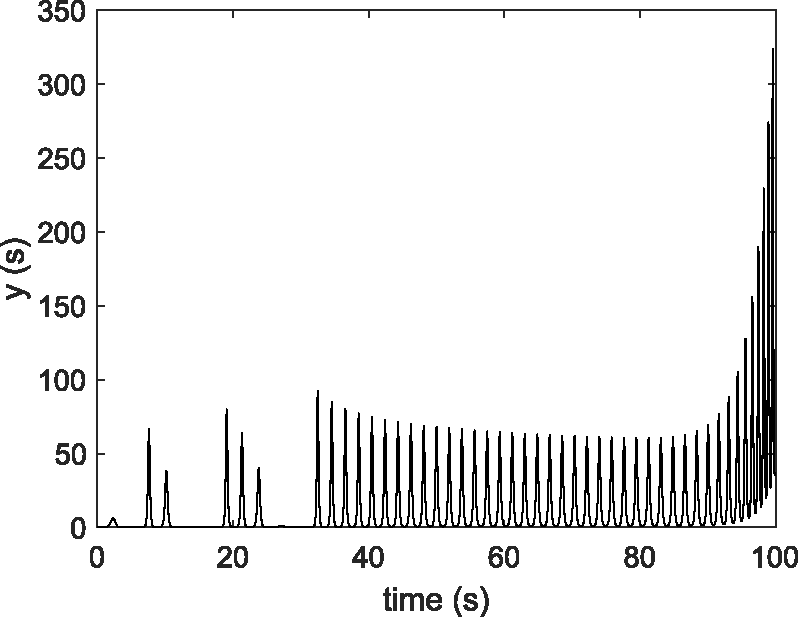
\includegraphics[scale=0.5]{figs/outParaAdown.pdf}
        \caption{Output signal in significant time for reduction in parameter $R_a$.}
        \label{fig:outParaAdown}
    \end{figure}
    \begin{figure}[H]
        \centering
        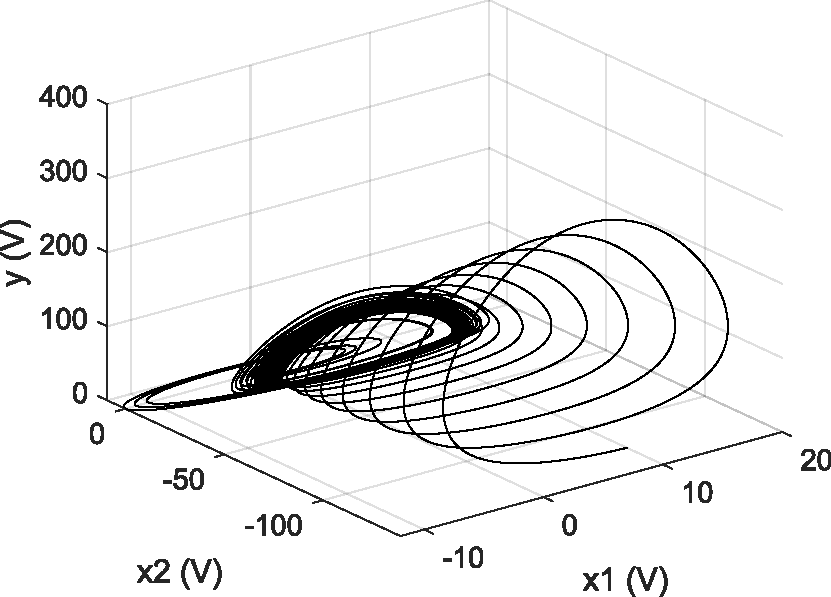
\includegraphics[scale=0.5]{figs/3dParaAdown.pdf}
        \caption{3D phase plot for the state variables for a significant reduction in parameter $R_a$.}
        \label{fig:3dParaAdown}
    \end{figure}
    
     Notice that, in the three-dimensional plot for the state variables, the trajectory starts to separate from the attractor; in the graph of $y$ against time, the output signal explodes and as $t$ increases, the output tends to infinity.
    
    Second, $R_a$ was set to $10000k\Omega$; this value was not found with the bisection method, since $R_a$ can take arbitrarily large numbers and all show the same output. In Figs. \ref{fig:outParaAup} and \ref{fig:3dParaAup} the behavior of the output in time and all three variables is shown.
    \begin{figure}[H]
        \centering
        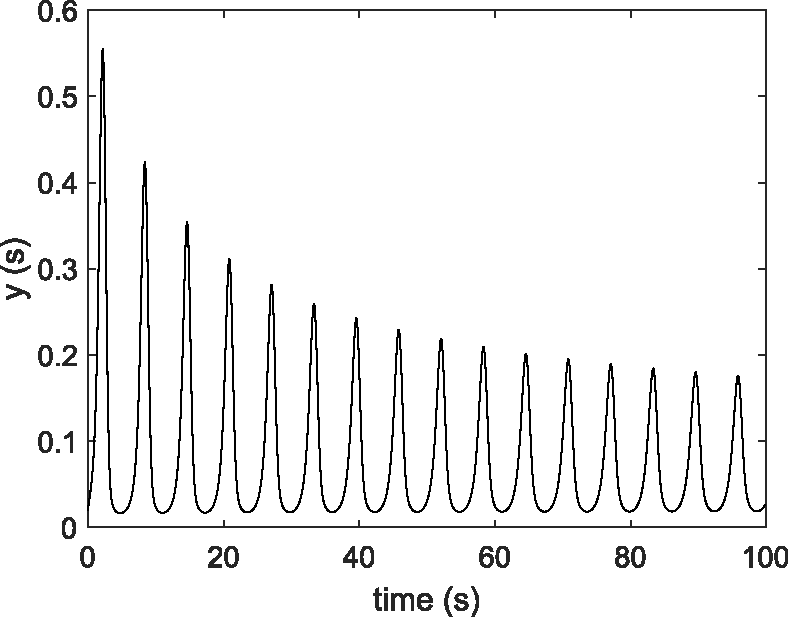
\includegraphics[scale=0.5]{figs/outParaAup.pdf}
        \caption{Output signal in time for a significant increment in parameter $R_a$.}
        \label{fig:outParaAup}
    \end{figure}
    \begin{figure}[H]
        \centering
        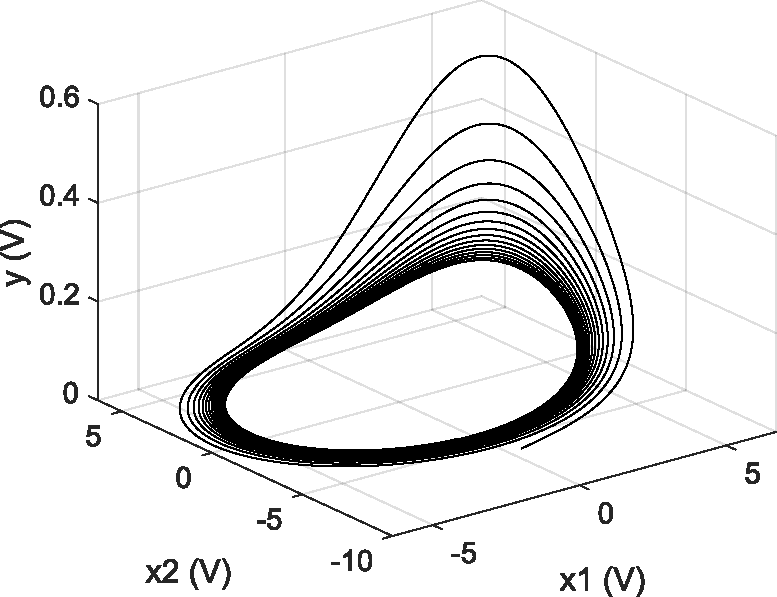
\includegraphics[scale=0.5]{figs/3dParaAup.pdf}
        \caption{3D phase plot for the state variables for an increment in parameter $R_a$.}
        \label{fig:3dParaAup}
    \end{figure}
    
    For the increment of $R_a$, the system behavior is periodic bounded by a decreasing signal, as the plot of $y$ against time shows. The 3D plots shows that the orbit falls into a decreasing loop.
    
    \subsubsection{Parameter \texorpdfstring{$R_c$}{Rc}}
    Following the idea from section \ref{subsubsec:ra}, the found minimum found value for $R_c$ is around $0.08400331675k\Omega$. In Figs. \ref{fig:outParaCdown} and \ref{fig:3dParaCdown} the behavior of the output in time and all three variables is shown.
    \begin{figure}[H]
        \centering
        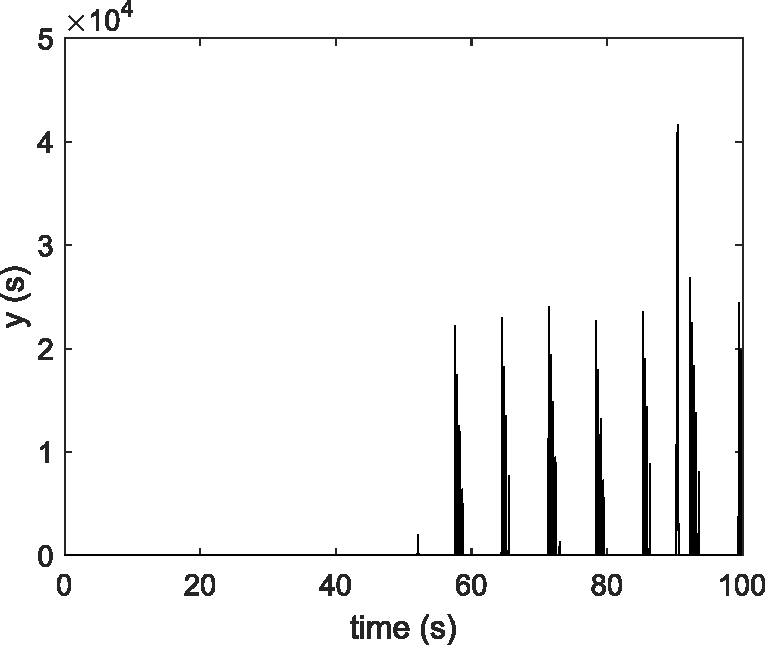
\includegraphics[scale=0.5]{figs/outParaCdown.pdf}
        \caption{Output signal in significant time for reduction in parameter $R_c$.}
        \label{fig:outParaCdown}
    \end{figure}
    \begin{figure}[H]
        \centering
        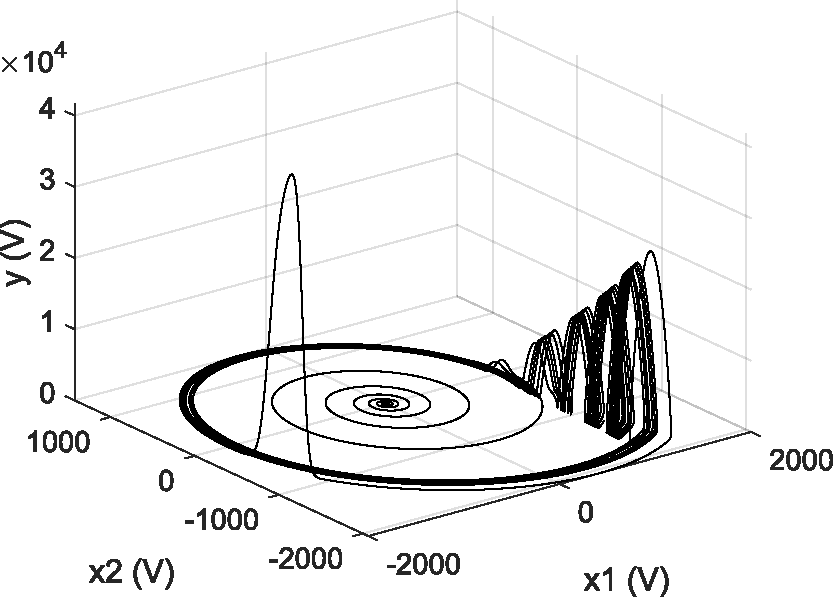
\includegraphics[scale=0.5]{figs/3dParaCdown.pdf}
        \caption{3D phase plot for the state variables for a significant reduction in parameter $R_c$.}
        \label{fig:3dParaCdown}
    \end{figure}
    
    Notice that, in the 3D plot, the opening of the attractor is shrinked, compared to higher values for $R_c$. The peaks in the output signal are much bigger than the standard values (order of $10^{4}$).
    
    For the increment maximum value in $R_c$, around $88.48868k\Omega$ was found with the bisection method. In Figs. \ref{fig:outParaCup} and \ref{fig:3dParaCup} the behavior of the output in time and all three variables is shown.
    \begin{figure}[H]
        \centering
        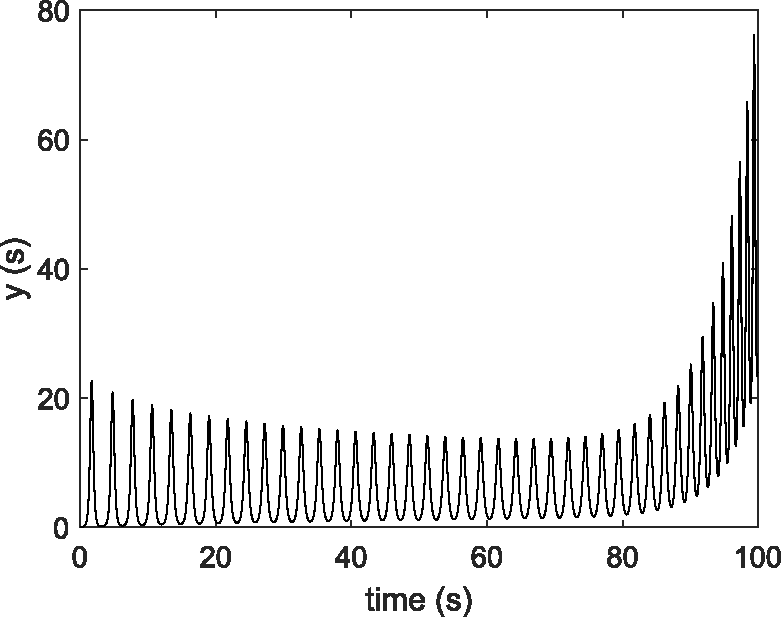
\includegraphics[scale=0.5]{figs/outParaCup.pdf}
        \caption{Output signal in time for a significant increment in parameter $R_c$.}
        \label{fig:outParaCup}
    \end{figure}
    \begin{figure}[H]
        \centering
        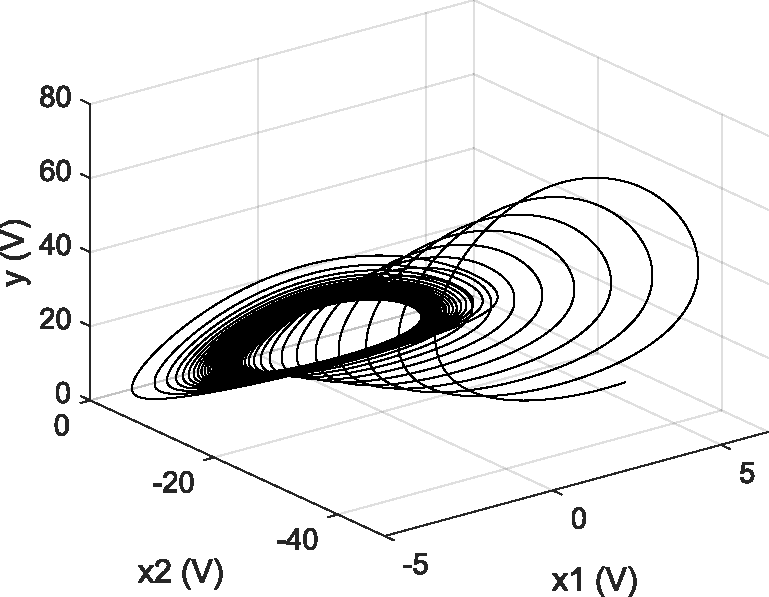
\includegraphics[scale=0.5]{figs/3dParaCup.pdf}
        \caption{3D phase plot for the state variables for an increment in parameter $R_c$.}
        \label{fig:3dParaCup}
    \end{figure}
    
    \subsection{Euler and Runge-Kutta Methods}\label{subsec:methods}
    A short comparison between the numerical methods was done, running simulations using Simulink's integrated methods and the manually programmed methods in Matlab for both fourth-order Runge-Kutta and Euler's method. The results are shown in Fig. \ref{fig:MethodMethod}.
    \begin{figure}[H]
        \centering
        \begin{subfigure}[b]{0.475\textwidth}
            \centering
            \includegraphics[scale=0.5]{figs/EulerEuler.pdf}
            \caption{}
        \end{subfigure}
        \vskip\baselineskip
        \begin{subfigure}[b]{0.475\textwidth}   
            \centering 
            \includegraphics[scale=0.5]{figs/RungeRunge.pdf}
            \caption{}
        \end{subfigure}
        \caption{System simulation with both Runge-Kutta and Euler methods using Simulink and programming the difference equation.}
        \label{fig:MethodMethod}
	\end{figure}
